% 图 84.3 —— 由 `checks/emit_hand.py` 自动拼出（probe 精测 + prims2 图元分解）
%%
% ⚠ 这是**稿子不是成品**：跑 `checks/checkhand.py 84.3` 看指标 + 看叠合图。
%%
%% ⚠ 待核：
%   · 本图 probe 报出阴影族 1 个 —— **本脚本不生成阴影**（要照原书手写）；prims2 的 strokes 里可能含阴影线，核对时留意别画重
%   · 可疑字形 2 项（空心圈 ⊙ 常被认成字母 o）—— 见文件末
%%
\documentclass[12pt]{standalone}
\usepackage{fontspec}
\setsansfont{Arial}
\newfontfamily\mfallback{DejaVu Sans}
\usepackage{tikz}
\usetikzlibrary{arrows.meta}
\begin{document}
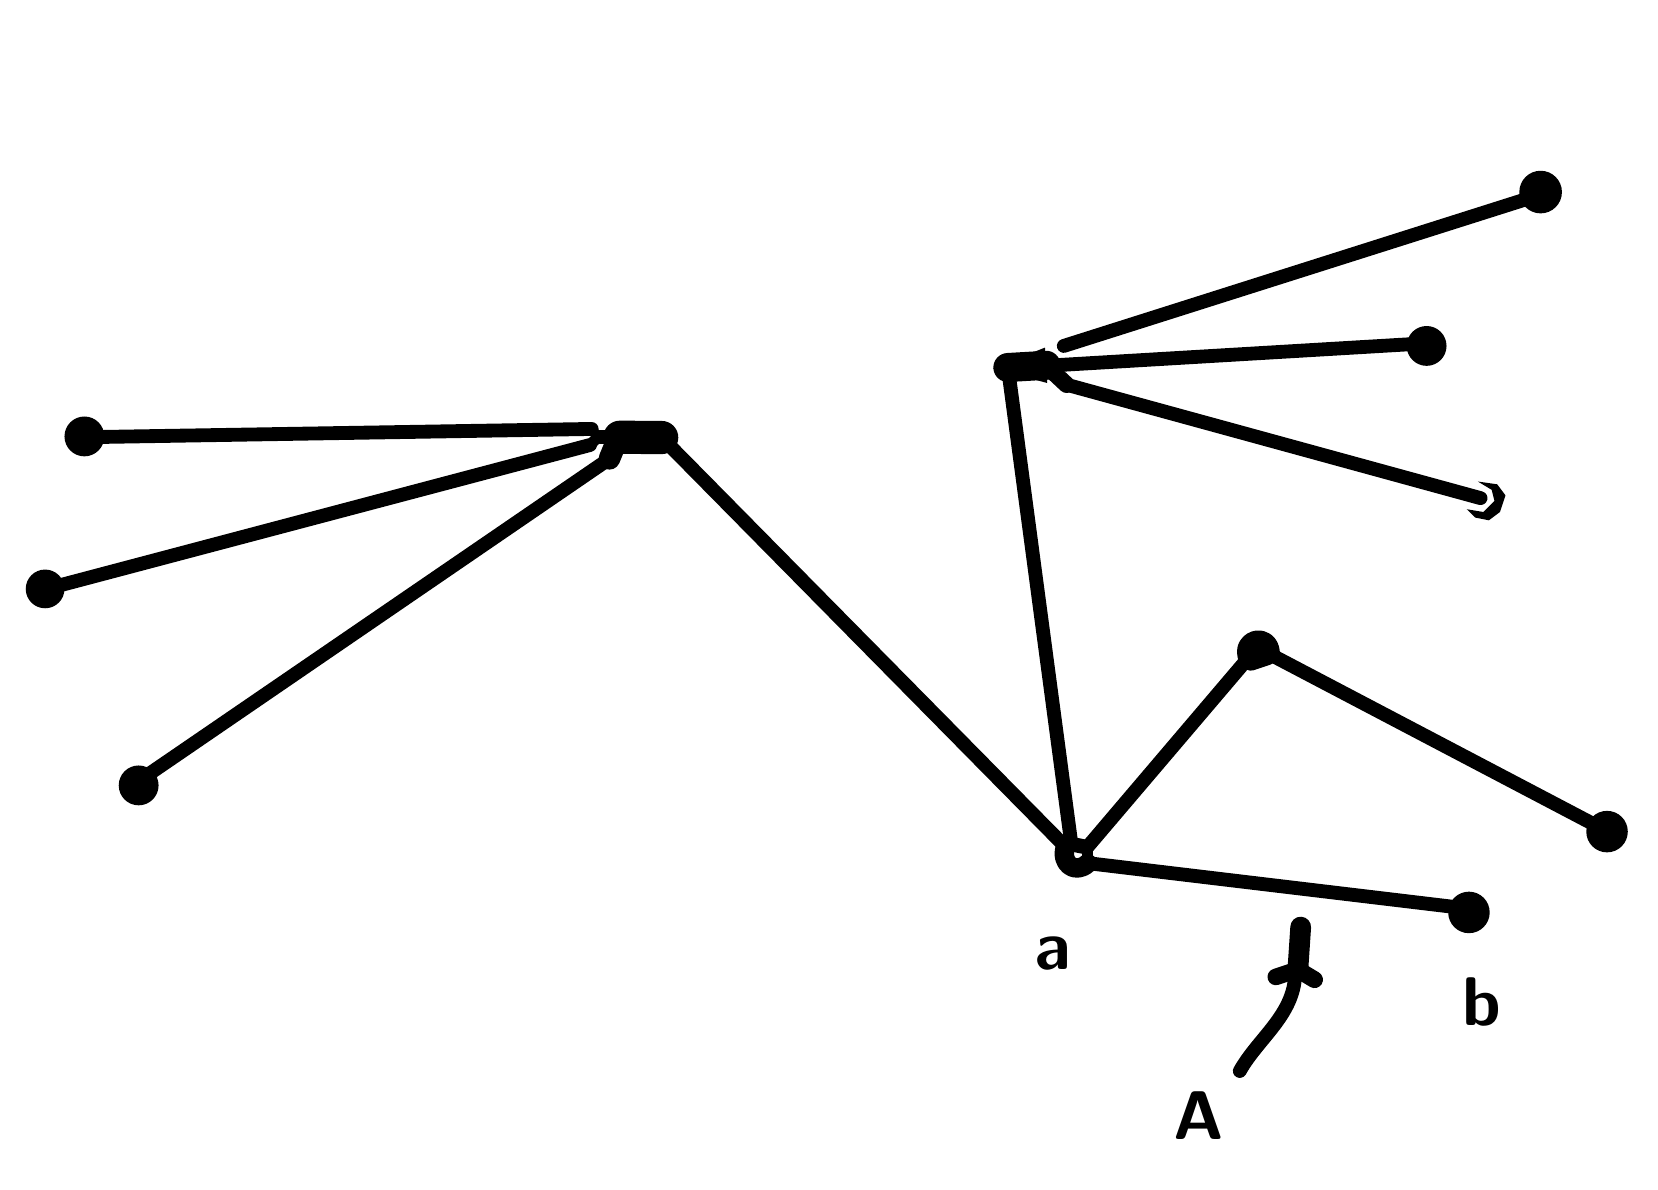
\begin{tikzpicture}[x=1pt, y=-1pt, line width=6.0pt, line cap=round, line join=round]

  %% ════ 填充区（prims2 的 fills）════
  \fill (524.0,164.0) -- (529.0,167.0) -- (530.0,171.0) -- (526.0,175.0) -- (520.0,174.0) -- (523.0,177.0) -- (528.0,178.0) -- (532.0,175.0) -- (534.0,169.0) -- (531.0,165.0) -- cycle;

  %% ════ 直线段（prims2 的 strokes）════
  \draw[line width=6.0pt] (457.0,341.0) -- (451.0,343.0);
  \draw[line width=5.0pt] (506.0,114.0) -- (371.0,122.0);
  \draw[line width=5.0pt] (570.0,290.0) -- (450.0,227.0);
  \draw[line width=6.1pt] (460.0,341.0) -- (465.0,344.0);
  \draw[line width=5.3pt] (382.0,296.0) -- (377.0,295.0);
  \draw[line width=5.0pt] (374.0,295.0) -- (229.1,148.1);
  \draw[line width=12.0pt] (229.1,148.1) -- (214.0,148.0);
  \draw[line width=4.0pt] (383.0,297.0) -- (383.0,301.0);
  \draw[line width=7.8pt] (213.0,149.0) -- (210.2,155.8);
  \draw[line width=5.0pt] (210.2,155.8) -- (39.0,273.0);
  \draw[line width=7.5pt] (460.0,325.0) -- (459.0,340.0);
  \draw[line width=3.0pt] (206.0,147.0) -- (203.8,145.0);
  \draw[line width=5.0pt] (203.8,145.0) -- (20.0,148.0);
  \draw[line width=5.0pt] (525.0,170.0) -- (375.4,129.0);
  \draw[line width=6.0pt] (375.4,129.0) -- (369.0,123.0);
  \draw[line width=5.0pt] (377.0,294.0) -- (354.2,122.8);
  \draw[line width=10.5pt] (354.2,122.8) -- (368.0,122.0);
  \fill (367.6,115.6) -- (368.4,128.4) -- (348.8,123.1) -- cycle;
  % （略）线段 (370.0,121.0)-(374.4,115.0) 线宽7.8 —— 是箭头头那一坨，已由箭头头代替
  \draw[line width=5.0pt] (374.4,115.0) -- (545.2,60.8);
  \draw[line width=4.0pt] (545.2,60.8) -- (548.0,58.0);
  \draw[line width=5.0pt] (384.0,302.0) -- (517.8,318.0);
  \draw[line width=3.8pt] (517.8,318.0) -- (521.0,320.0);
  \draw[line width=5.0pt] (440.0,229.0) -- (383.0,296.0);
  \draw[line width=5.0pt] (207.0,148.0) -- (212.0,148.0);
  \draw[line width=5.0pt] (6.0,203.0) -- (203.2,150.8);
  \draw[line width=4.0pt] (203.2,150.8) -- (206.0,148.0);
  \draw[line width=6.7pt] (448.0,227.0) -- (442.0,229.0);

  %% ════ 曲线（prims2 的 curves —— 三段式，坐标同为 (y,x)）════
  \draw[line width=5.0pt] (458.0,342.0) .. controls (457.6,356.8) and (444.6,365.2) .. (438.0,377.0);
  \draw[line width=7.0pt] (375.0,296.0) .. controls (373.0,301.9) and (378.4,306.2) .. (383.0,302.0);
  \draw[line width=7.0pt] (449.0,226.0) .. controls (448.6,218.4) and (438.1,220.6) .. (441.0,228.0);

  %% ════ 实心点 ════
  \fill (546.7,59.4) circle (7.7);
  \fill (505.5,115.0) circle (7.2);
  \fill (20.5,147.7) circle (7.2);
  \fill (6.3,202.8) circle (7.0);
  \fill (40.1,273.8) circle (7.2);
  \fill (570.7,290.5) circle (7.5);
  \fill (520.8,319.7) circle (7.5);

  %% ════ 标签（probe 直接给的 \node 行）════
  %% ⚠ 全部补了 fill=white：文字在最上层，否则与曲线交叉干扰
     \node[anchor=center,inner sep=0pt,fill=white,font=\fontsize{35.8}{44.7}\selectfont] at (370.7,334.8) {\textsf{\textbf{\textit{a}}}};   % box(361,323,17,20)
     \node[anchor=center,inner sep=0pt,fill=white,font=\fontsize{34.7}{43.4}\selectfont] at (525.4,351.9) {\textsf{\textbf{\textit{b}}}};   % box(514,338,20,25)
     \node[anchor=center,inner sep=0pt,fill=white,font=\fontsize{33.9}{42.4}\selectfont] at (423.1,393.1) {\textsf{\textbf{\textit{A}}}};   % box(409,380,22,25)

  % 钉死画布：否则超出的图元/控制点会把页面撑大，1:1 回比就失准
  \pgfresetboundingbox
  \path[use as bounding box] (0,0) rectangle (579,410);
\end{tikzpicture}
\end{document}

% ⚠ 待核清单（probe 拿不准，人眼过一遍）：
%   · 未识别/跳过：⑤ 跳过/未识别的字形
%   · 未识别/跳过：box(437,322,31,57)
